\documentclass[10pt, a4paper]{scrartcl}

%\usepackage{qrcode}

\usepackage{vorschule}
\usepackage[
	typ=ab,
	fach=Informatik,
	lerngruppe={EF},
	nummer=8,
	module={Symbole,Lizenzen},
	seitenzahlen=keine,
	farbig,
	lizenz=cc-by-nc-sa-4,
]{schule}

\usepackage[
	kuerzel=Ngb,
	reihe={Objektorientierte Programmierung},
	version={2019-12-16},
]{ngbschule}

\clearscrheadings

\begin{document}

\begin{wrapfig}
	\begin{wrapfigure}{r}{0pt}
		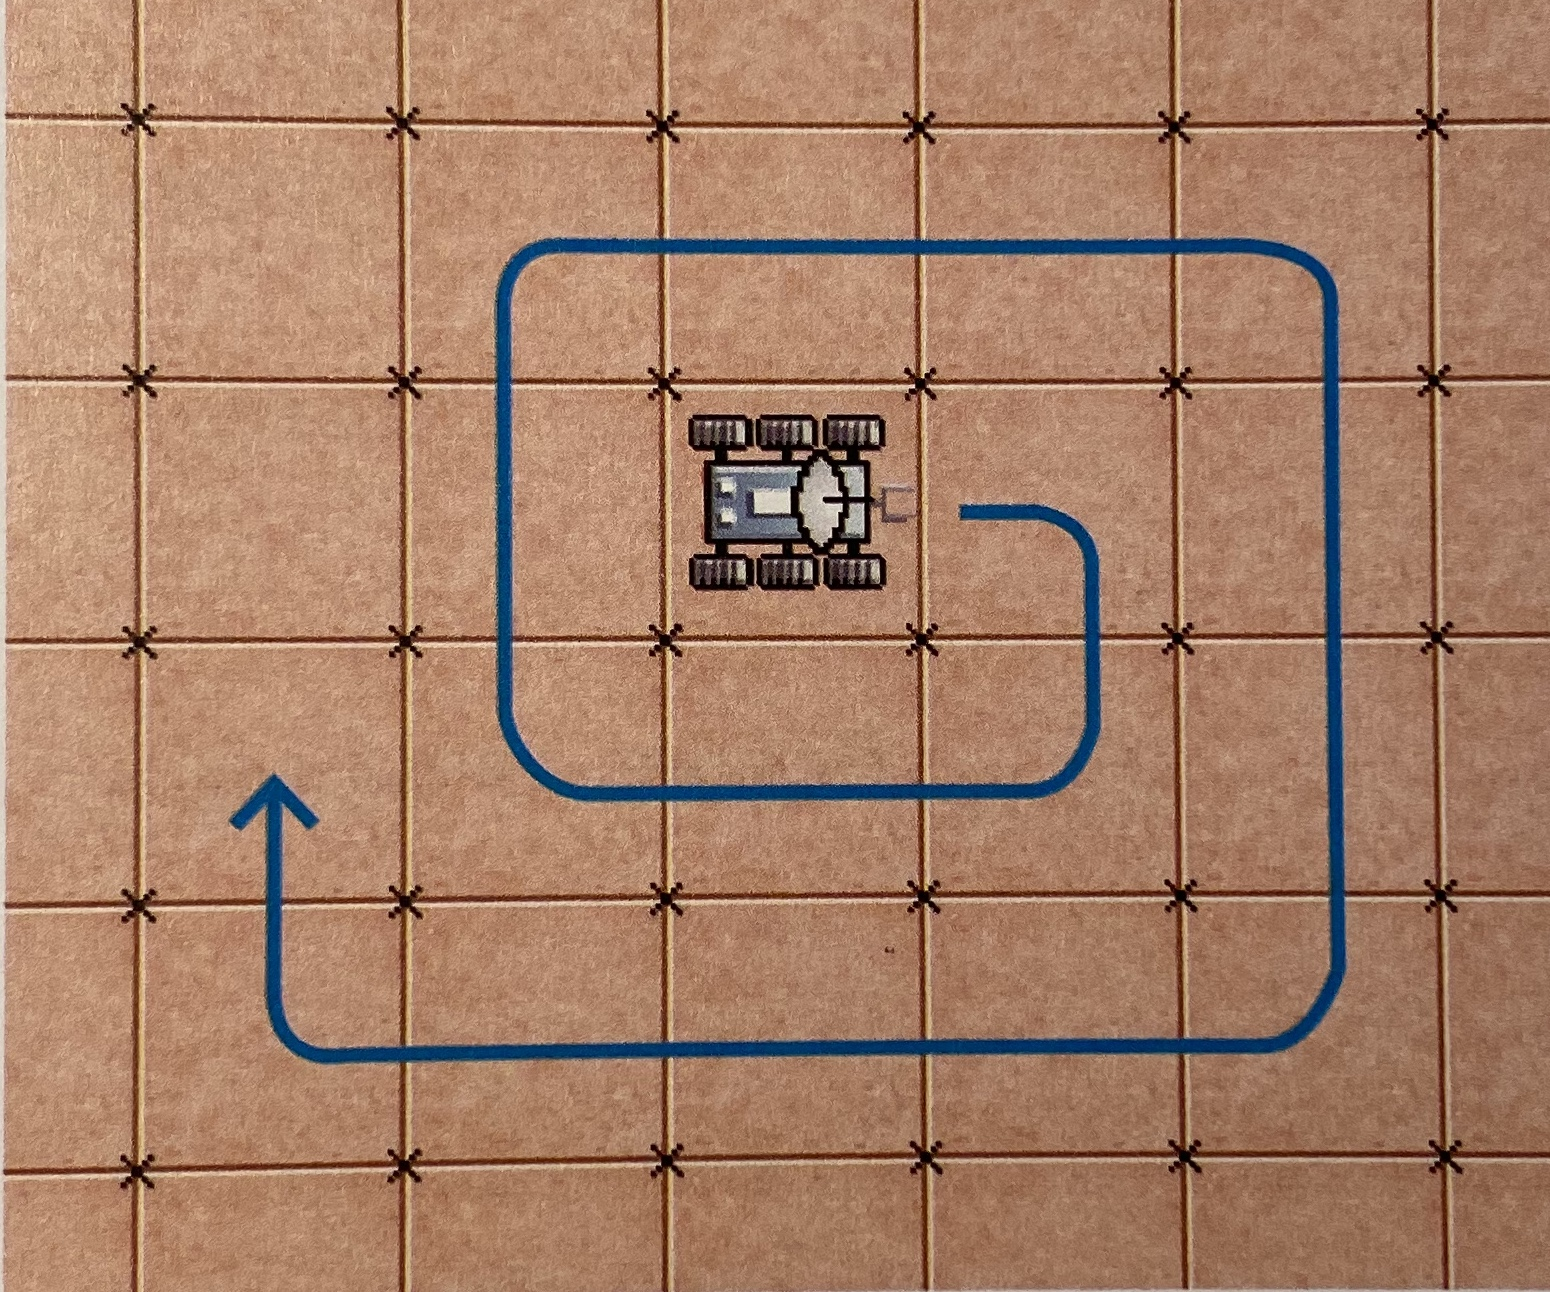
\includegraphics[width=4cm]{EF-AB.8-Abb_Spirale}
	\end{wrapfigure}
	
	\subsubsection*{Aufgabe 4}
	Implementiert eine Methode \code{int sucheGestein( int runden )}, die den Rover von seiner Startposition aus in einer größer werdenden Spirale nach Gesteinen suchen lässt. Der \emph{Parameter} \code{runden} soll angeben, wie viele Runden der Rover auf seiner Suche fährt, bevor er anhält. Am Ende soll die Anzahl der gefundenen Steine \emph{zurück gegeben} werden.
\end{wrapfig}

\vspace{1cm}
\titlerule
\vspace{1cm}

\begin{wrapfig}
	\begin{wrapfigure}{r}{0pt}
		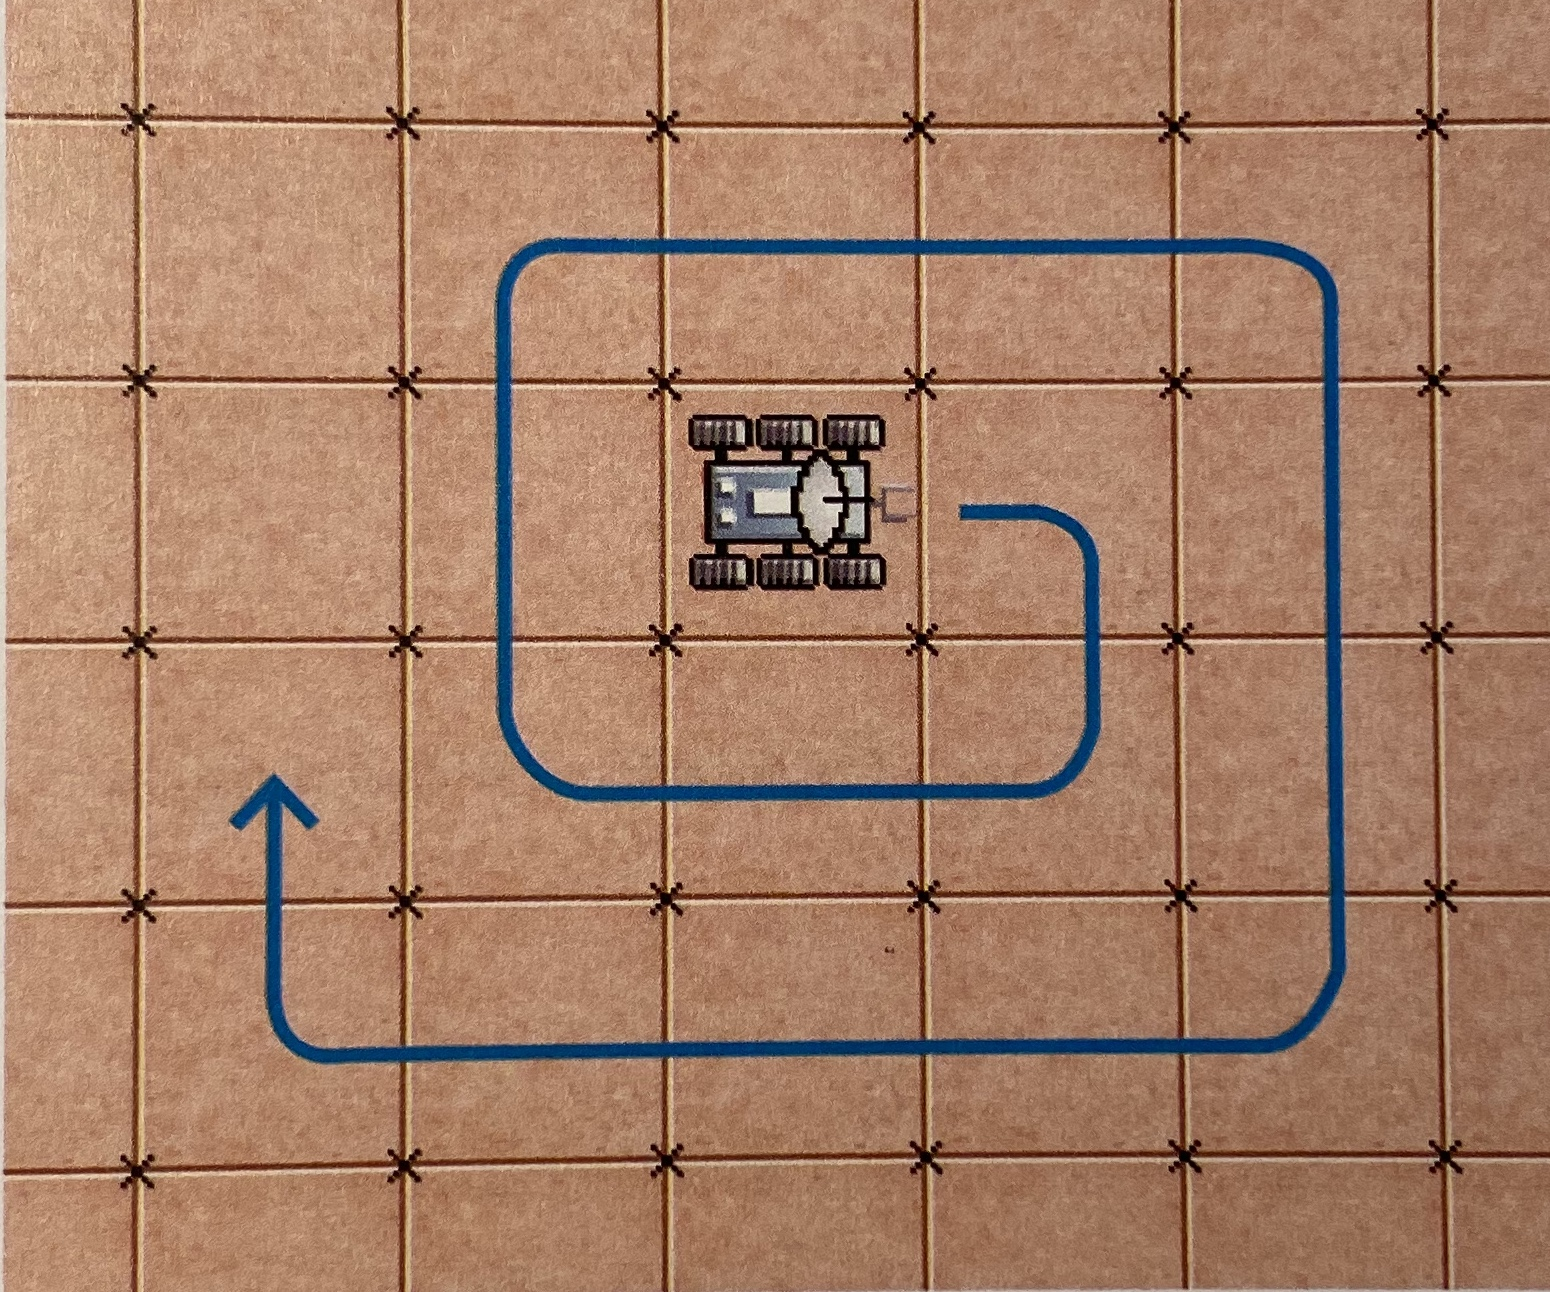
\includegraphics[width=4cm]{EF-AB.8-Abb_Spirale}
	\end{wrapfigure}
	
	\subsubsection*{Aufgabe 4}
	Implementiert eine Methode \code{int sucheGestein( int runden )}, die den Rover von seiner Startposition aus in einer größer werdenden Spirale nach Gesteinen suchen lässt. Der \emph{Parameter} \code{runden} soll angeben, wie viele Runden der Rover auf seiner Suche fährt, bevor er anhält. Am Ende soll die Anzahl der gefundenen Steine \emph{zurück gegeben} werden.
\end{wrapfig}

\vspace{1cm}
\titlerule
\vspace{1cm}

\begin{wrapfig}
	\begin{wrapfigure}{r}{0pt}
		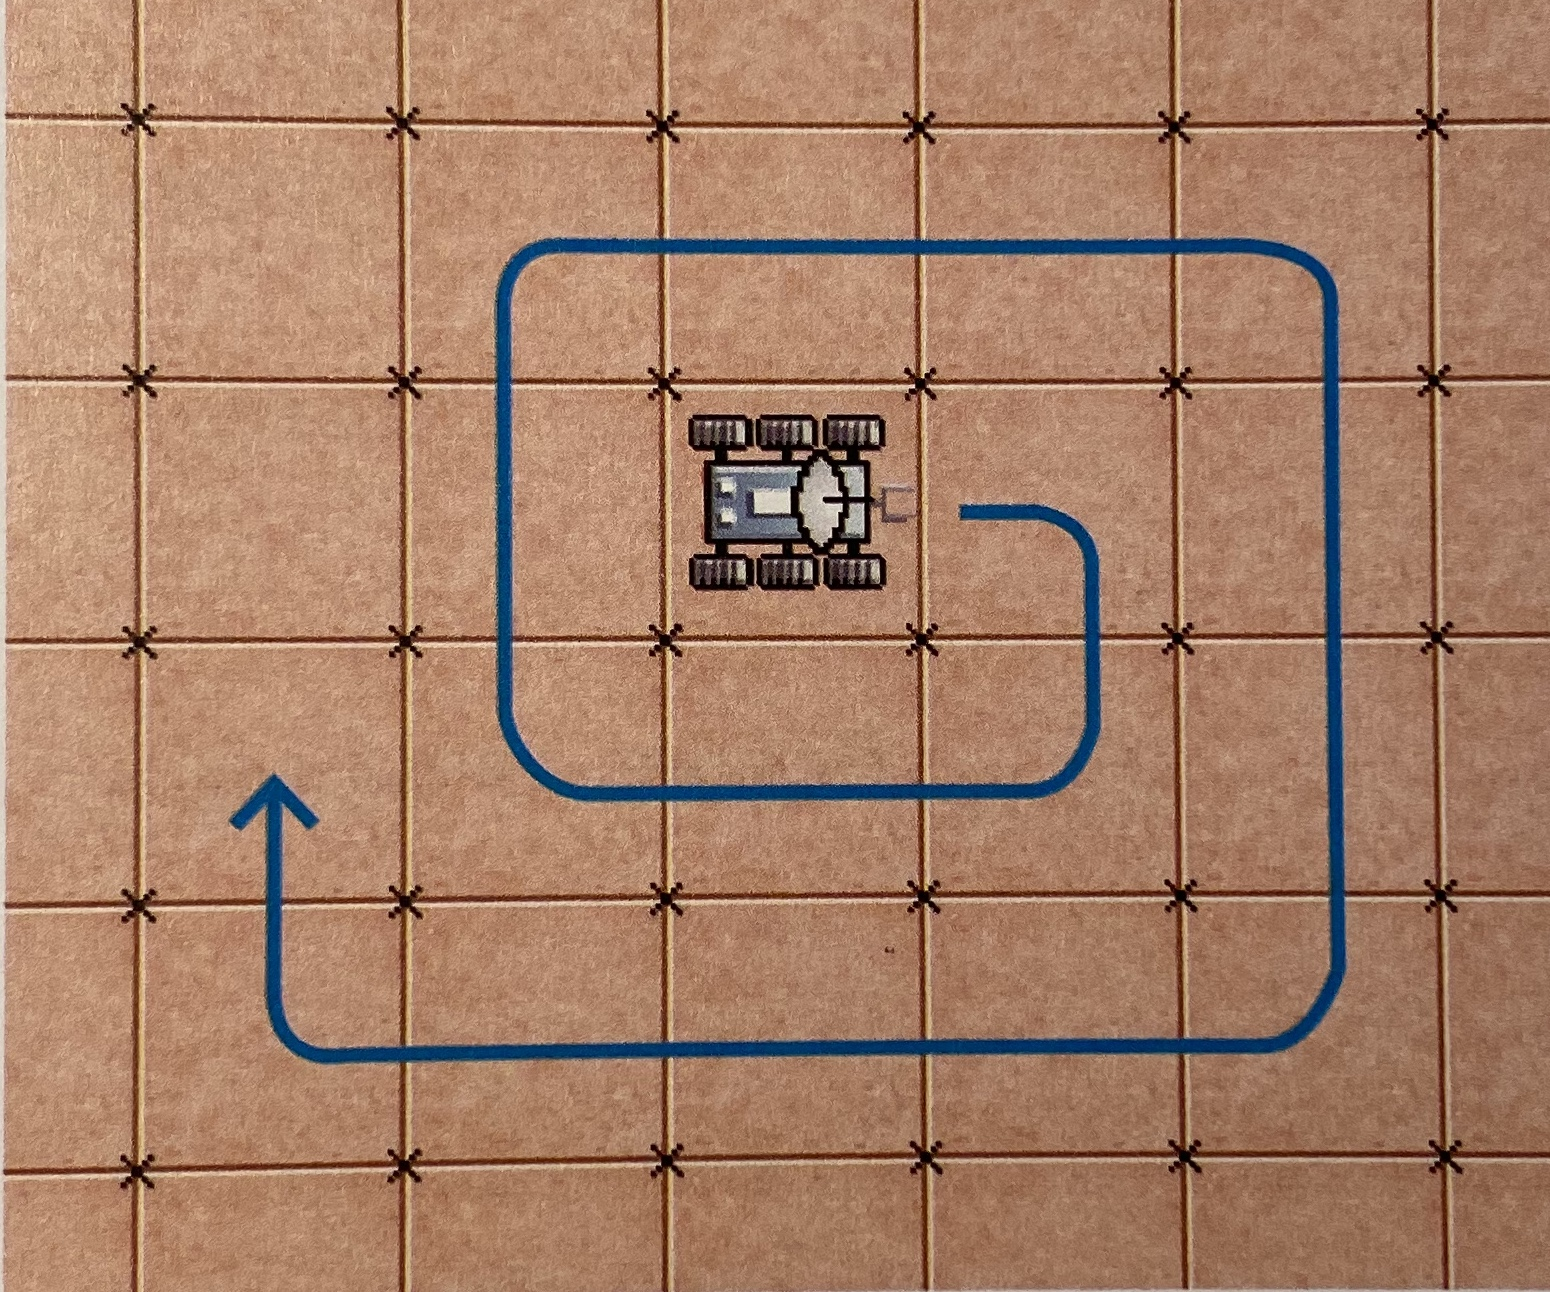
\includegraphics[width=4cm]{EF-AB.8-Abb_Spirale}
	\end{wrapfigure}
	
	\subsubsection*{Aufgabe 4}
	Implementiert eine Methode \code{int sucheGestein( int runden )}, die den Rover von seiner Startposition aus in einer größer werdenden Spirale nach Gesteinen suchen lässt. Der \emph{Parameter} \code{runden} soll angeben, wie viele Runden der Rover auf seiner Suche fährt, bevor er anhält. Am Ende soll die Anzahl der gefundenen Steine \emph{zurück gegeben} werden.
\end{wrapfig}

\vspace{1cm}
\titlerule
\vspace{1cm}

\begin{wrapfig}
	\begin{wrapfigure}{r}{0pt}
		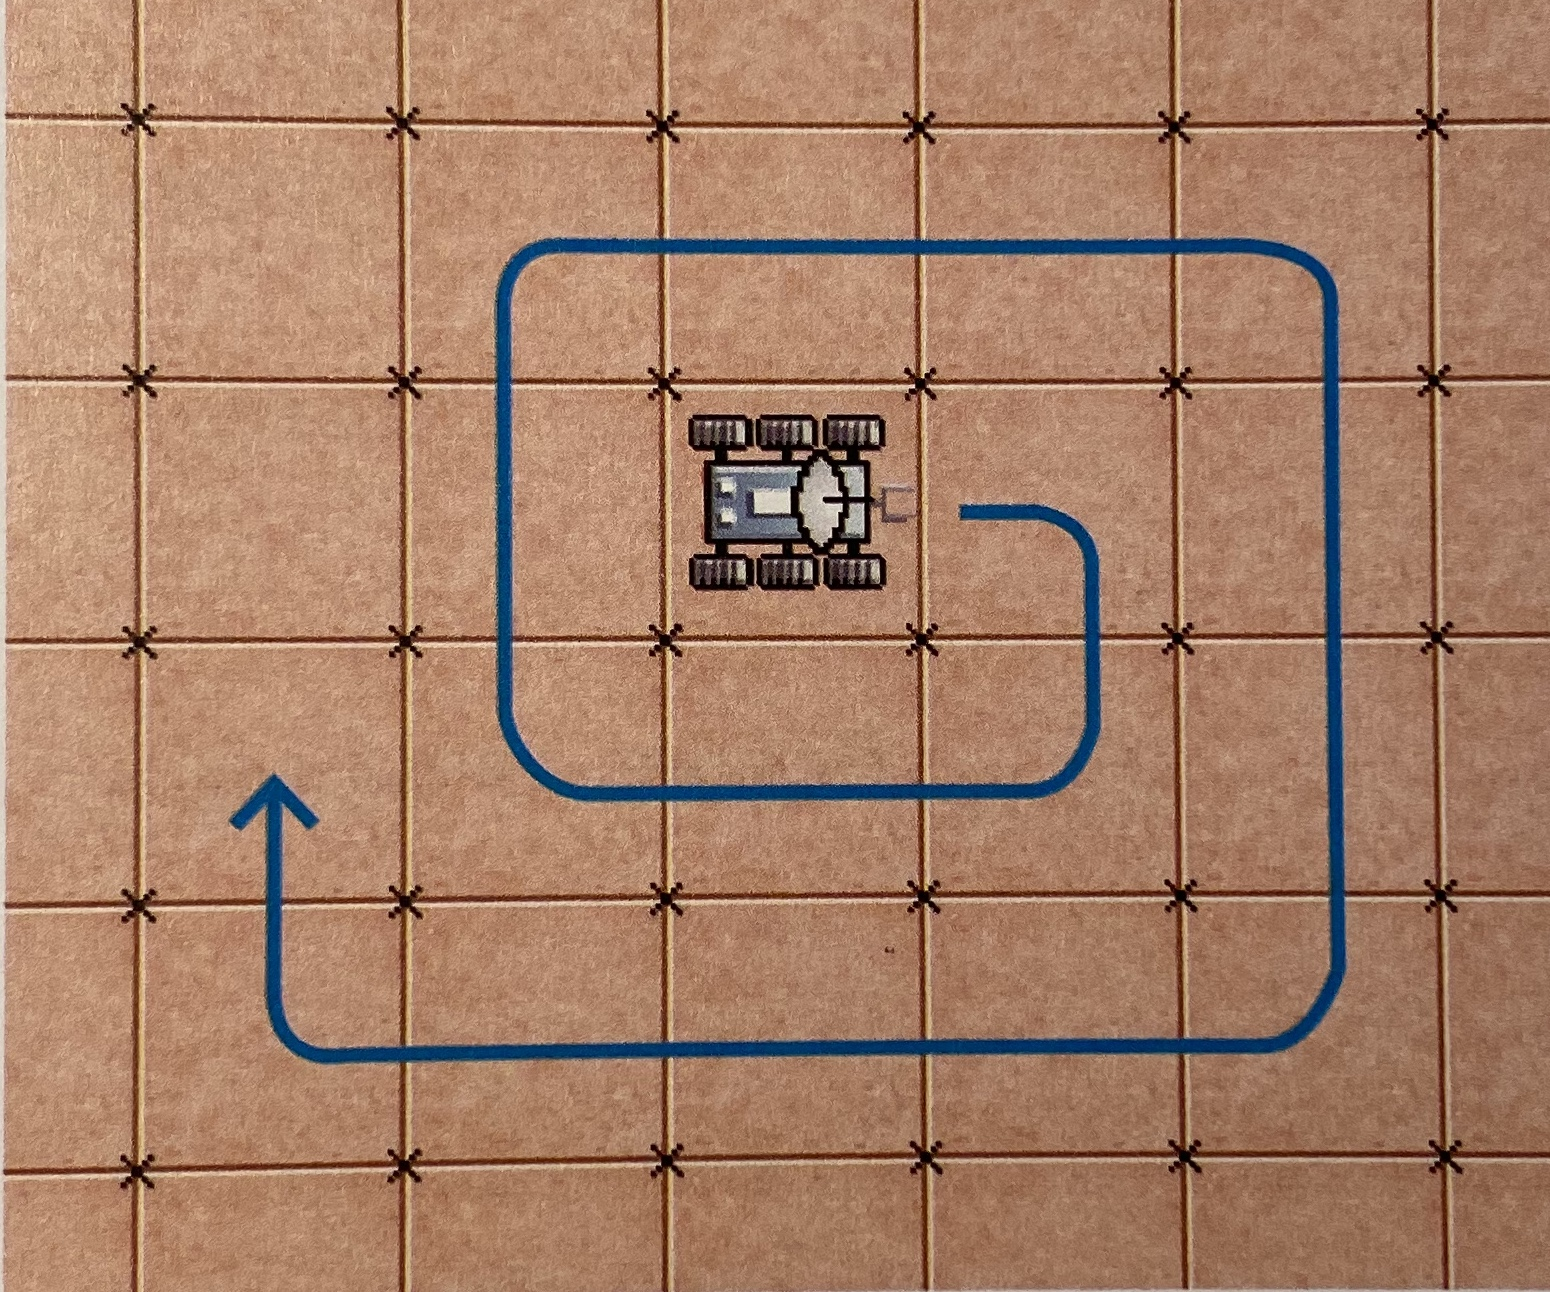
\includegraphics[width=4cm]{EF-AB.8-Abb_Spirale}
	\end{wrapfigure}
	
	\subsubsection*{Aufgabe 4}
	Implementiert eine Methode \code{int sucheGestein( int runden )}, die den Rover von seiner Startposition aus in einer größer werdenden Spirale nach Gesteinen suchen lässt. Der \emph{Parameter} \code{runden} soll angeben, wie viele Runden der Rover auf seiner Suche fährt, bevor er anhält. Am Ende soll die Anzahl der gefundenen Steine \emph{zurück gegeben} werden.
\end{wrapfig}

\end{document}
